\subsection{Effect of Cache Partitioning}

\begin{figure}[h]
  \centering
  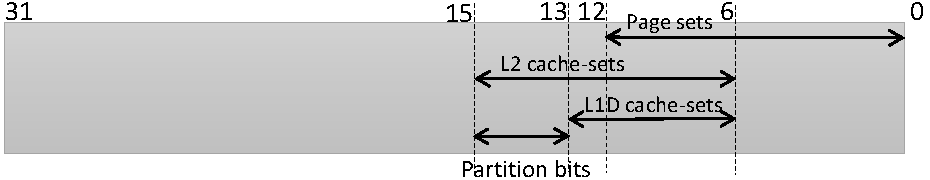
\includegraphics[width=\textwidth]{figs/cache-mapping}
  \caption{A memory mapping of the cache sets for the Broadcom 
BCM2837 processor used in the Raspberry Pi 3 Model B.}
  \label{fig:cache-mapping}
\end{figure}

\begin{figure}[h]
  \centering
  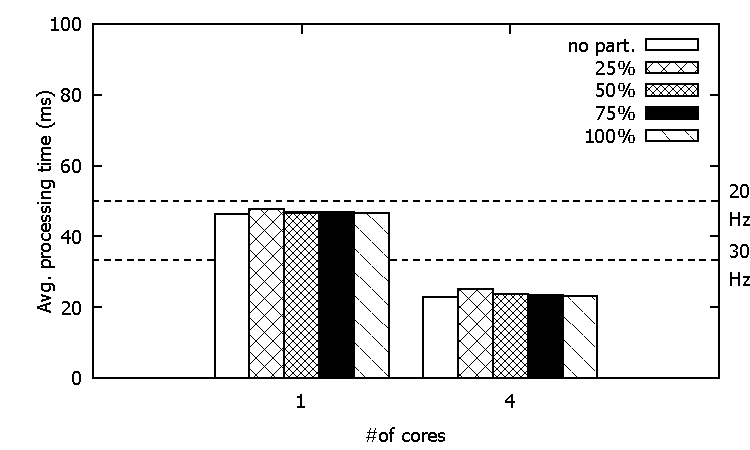
\includegraphics[width=.7\textwidth]{figs/palloc_multicore}
  \caption{Average control loop execution time vs.  % of L2 cache
    L2 cache partition size.}
  \label{fig:palloc_multicore}
\end{figure}

%% \begin{figure}[h]
%%   \centering
%%   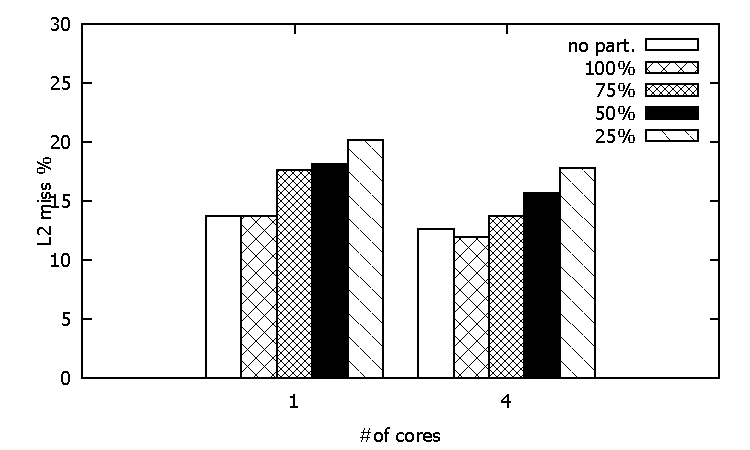
\includegraphics[width=.7\textwidth]{figs/palloc_multicore_l2missrate}
%%   \caption{L2 miss rate impact of limiting the amount of L2 cache space
%%   available to the DNN.}
%%   \label{fig:palloc_multicore_l2missrate}
%% \end{figure}

%% \begin{figure}[h]
%%   \centering
%%   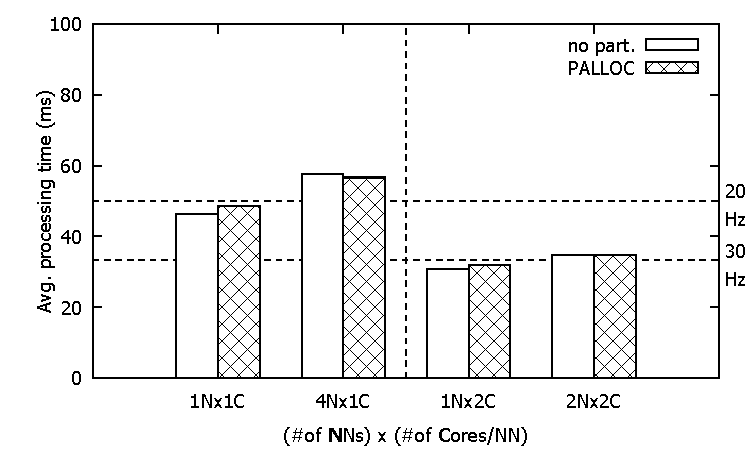
\includegraphics[width=.7\textwidth]{figs/palloc_multimodel}
%%   \caption{Timing impact of co-scheduling multiple DNNs when cache 
%% partitioning is enabled.}
%%   \label{fig:palloc_multimodel}
%% \end{figure}

\begin{figure}[h]
  \centering
  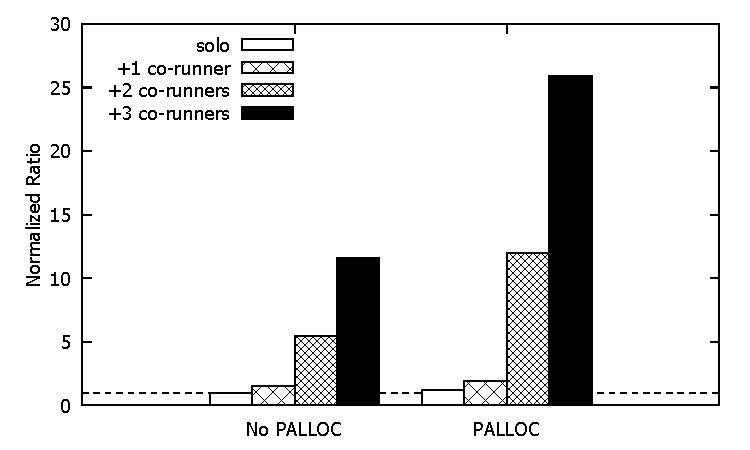
\includegraphics[width=.7\textwidth]{figs/palloc_bandwidth_exectime}
  \caption{Timing impact of co-scheduling memory intensive co-runners 
when cache partitioning is enabled.}
  \label{fig:palloc_bandwidth_exectime}
\end{figure}

%% \begin{figure}[h]
%%   \centering
%%   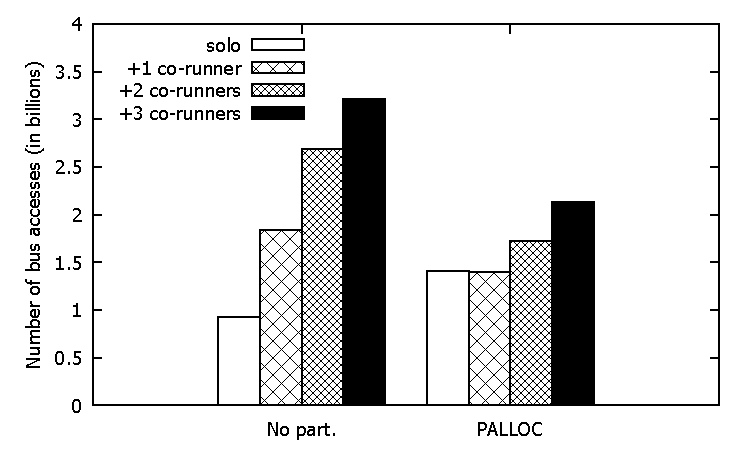
\includegraphics[width=.7\textwidth]{figs/palloc_bandwidth_modelbus}
%%   \caption{Model bus access impact of co-scheduling memory intensive co-runners 
%% when cache partitioning is enabled.}
%%   \label{fig:palloc_bandwidth_modelbus}
%% \end{figure}

%% \begin{figure}[h]
%%   \centering
%%   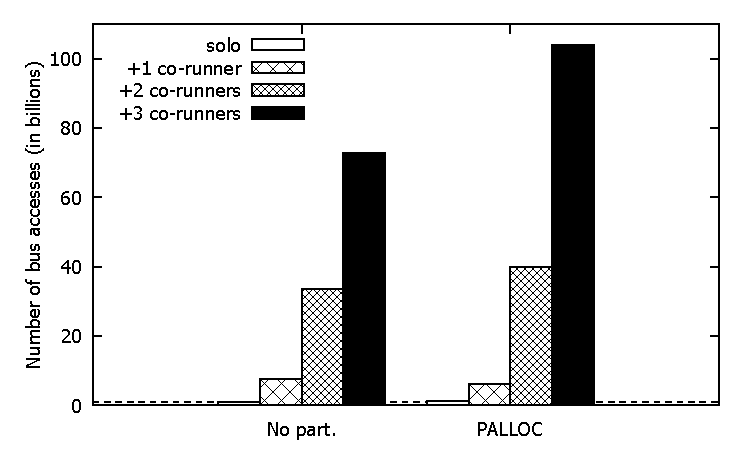
\includegraphics[width=.7\textwidth]{figs/palloc_bandwidth_bus}
%%   \caption{Total bus access impact of co-scheduling memory intensive co-runners 
%% when cache partitioning is enabled.}
%%   \label{fig:palloc_bandwidth_bus}
%% \end{figure}

%% \begin{figure}[h]
%%   \centering
%%   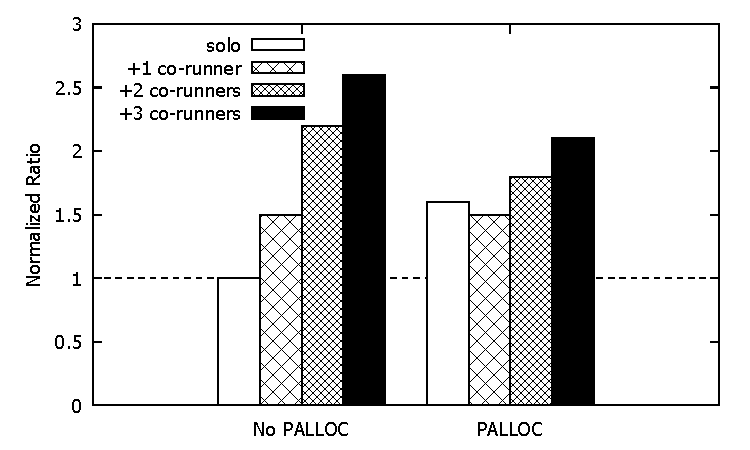
\includegraphics[width=.7\textwidth]{figs/palloc_bandwidth_l2missrate}
%%   \caption{L2 miss rate impact of co-scheduling memory intensive co-
%% runners when cache partitioning is enabled.}
%%   \label{fig:palloc_bandwidth_l2missrate}
%% \end{figure}

In order to validate the effectiveness of cache partitioning, we patch
the kernel with PALLOC~\cite{yun2014rtas}, which is a kernel-level
color-aware page allocator, supporting cache partitioning. 
Figure~\ref{fig:cache-mapping} shows the physical address mapping of
Raspberry Pi3's BCM2837 processor. We use the bit 12, 13, 14 for
coloring, which results in 8 page colors.

%% determine if the DNN is mostly affected by the DRAM 
%% controller, we partition the L2 cache of the Pi3 and reperform the 
%% same experiments to see if there are any noticable changes. For the 
%% partition, we employ PALLOC~\cite{yun2014rtas}, a color-based page 
%% allocator that works on the kernel level.

%% For the bit mask, we select 
%% bits 12, 13 and 14 as they can be used to access the L2 cache,
%% as can be seen by Figure \ref{fig:cache-mapping}.
%% This results in 
%% 2\textsuperscript{3} = 8 colors, which we then assign to the Pi3's 
%% physical cores such that each core has two unique colors (colors 0 
%% and 1 are assigned to core 0, colors 2 and 3 are assigned to core 1, 
%% etc.). In the case of bit 12, since we use 2 colors for each partition,
%% the L1 Data cache is not partitioned in our experiments.

In the first experiment, we investigate the cache space sensitivity of
the DeepPicar's DNN-based control loop. Using PALLOC, we create 4
different cgroups which are configured to use 2, 4,
6, 8 colors (25\%, 50\%, 75\%, 100\% of the L2 cache
space, respectively). We then execute the control loop on each cache
partition (cgroup) and measure the average processing time. 

If performance improves as a result of partitioning the shared cache 
then we know that the DNN, to some extent, relies on shared cache 
performance in addition to shared DRAM performance. On the other 
hand, if there is no improvement in performance, then it can be 
observed that the shared memory is more critical to the performance 
of the DNN.

We run the DNN model with different amounts of L2 cache being
available based on the number of colors being used. For example, if two 
colors are used, then 25\% of the L2 cache is available, whereas if all 
8 colors are used, 100\% of the L2 cache is available. Particularly, we 
test the performance of the model when it utilizes a single core and
all four of the available cores. The results can be seen in 
\ref{fig:palloc_multicore}. As expected, the amount of L2 cache 
available to the model does not result in any significant changes in 
performance. This can also be seen by the L2 miss rates of the model 
seen in \ref{fig:palloc_multicore_l2missrate}. As more cache space 
becomes avaiable, the percentage of L2 misses decreases, which doesn't 
affect the real-time performance of the DNN. As such, we find that a 
single model is not sensitive to the shared L2 cache.

We also co-schedule multiple models to see how cache partitioning affects
interference between them. Each model uses an equal number of colors, and
are thus given equal amounts of L2 cache space, and there is no overlap
in the colors used, so no L2 cache is shared between models. As can be 
seen in \ref{fig:palloc_multimodel}, the performance of the models 
remains the same as when no cache partitioning was employed. Based of 
these results, we find that contention for the L2 cache is not the main
source of interference between multiple DNN models.

Finally, we run a single model alongside memory intensive co-runners 
again, but ensure that each task is given equal amounts of L2 cache space.
For this, we assign two colors to each task, regardless of the number of
tasks being scheduled. As a result, the entire cache is not utilized in
experiments with less than four tasks. The results can be seen in Figure
\ref{fig:palloc_bandwidth_exectime}. With zero or one co-runners, the DNN
performance doesnt't change relative to when the cache wasn't partitioned.
However, we find that with two or more co-runners, DNN performance becomes
worse. In the case of two co-runners, average control loop time increases
by 66.31 ms, or 26\%, and with three co-runners, the average time
is 265.64 ms, of 49\%, greater.
At the same time, though, the L2 miss rates of the model don't correlate 
to the timing increases seen, as is shown in 
\ref{fig:palloc_bandwidth_l2missrate}. Instead, we find that the number
of bus accesses increases when cache partitions are used, and they mirror
the timing increases of the model. This can be seen in Figure 
\ref{fig:palloc_bandwidth_bus}. These additional bus accesses are
most likely caused by the L2 prefetcher, as it can generate additional bus
accesses that aren't counted as L2 misses. As a result, we find that cache
partitioning is detrimental to the performance of the DNN so long as the 
L2 prefetcher is enabled (we have not yet found a way to disable it on
the Pi 3). Furthermore, no cache sensitivity was displayed by the model,
thus showing that the performance of the L2 cache is not vital for DNN 
performance when co-runners are introduced.

By partitioning the shared L2 cache, we find that no noticable 
improvements are gained and that performance remains consistent, or 
decreases, depending on the circumstances. In all experiements, the DNN
shows no sensitivity to the shared L2 cache. As a result, we conclude 
that cache partitioning is not an effective isolation mechanism, and that 
the performance of the shared DRAM controller is of greater importance 
to the real-time efficiacy of the DeepPicar.
